\documentclass{beamer}

\usepackage[portuguese]{babel}
\usepackage[utf8]{inputenc}
\usepackage{hyperref}
\usepackage[style=brazilian]{csquotes}
\usepackage{subcaption}
\usepackage{xcolor}

\def\signed #1{{\leavevmode\unskip\nobreak\hfil\penalty50\hskip1em
  \hbox{}\nobreak\hfill #1%
  \parfillskip=0pt \finalhyphendemerits=0 \endgraf}}

\newsavebox\mybox
\newenvironment{aquote}[1]
  {\savebox\mybox{#1}\begin{quote}\openautoquote\hspace*{-.7ex}}
  {\unskip\closeautoquote\vspace*{1mm}\signed{\usebox\mybox}\end{quote}}

\usetheme{boxes}

\title{Duckievillage: OpenAI Gym Duckietown na USP
\\\vspace{1.0cm}\centering
\includegraphics[height=0.35\textheight]{../imgs/duckieusp.png}
\vspace{-0.5cm}}
\date{}
\institute{\small MAC0318 - Introdução à Programação de Robôs Móveis\\~\\\scriptsize Instituto de
Matemática e Estatística (IME)\\Universidade de São Paulo (USP)}

\begin{document}

\begin{frame}
  \titlepage
\end{frame}

\section{Duckietown}

\begin{frame}
  \frametitle{Duckietown}

  Robótica com patinhos.
  \vspace{1cm}

  \begin{figure}
    \begin{subfigure}{0.49\linewidth}
      \centering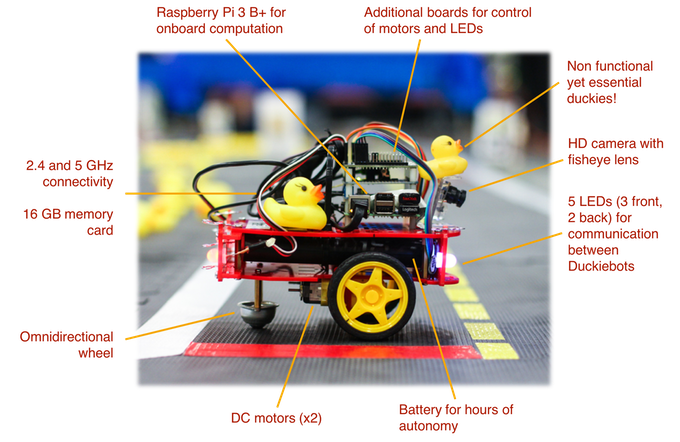
\includegraphics[width=\textwidth]{../imgs/duckiebot.png}
    \end{subfigure}
    \begin{subfigure}{0.49\linewidth}
      \centering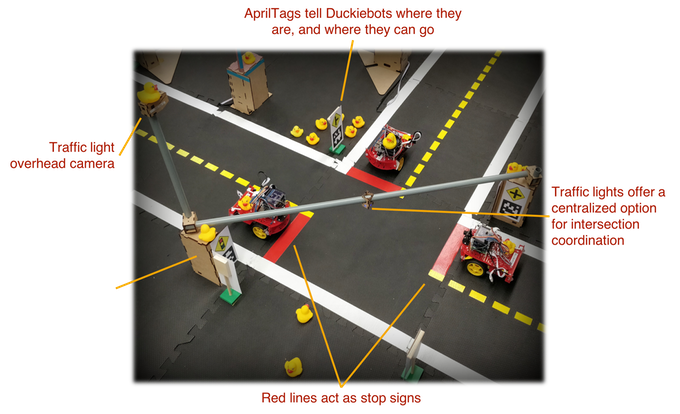
\includegraphics[width=\textwidth]{../imgs/intersection.png}
    \end{subfigure}
  \end{figure}
  \begin{center}
    \textcolor{blue}{
      \href{https://www.kickstarter.com/projects/163162211/duckietown-a-playful-road-to-learning-robotics-and/description}{Videos}
    }
  \end{center}
  \vspace{1cm}

  \url{https://www.duckietown.org/}
\end{frame}

\section{OpenAI Gym}

\begin{frame}
  \frametitle{OpenAI Gym}

  \begin{aquote}{http://gym.openai.com/}
    Gym is a toolkit for developing and comparing reinforcement learning algorithms. It supports
    teaching agents everything from walking to playing games like Pong or Pinball.
  \end{aquote}

  \vspace{3cm}
  \textcolor{red}{Exemplos:} \url{http://gym.openai.com/envs}
\end{frame}

\section{Gym-Duckietown}

\begin{frame}
  \frametitle{Gym-Duckietown}

  Simulador do Duckietown no OpenAI Gym.
  \vspace{0.5cm}

  \begin{figure}
    \centering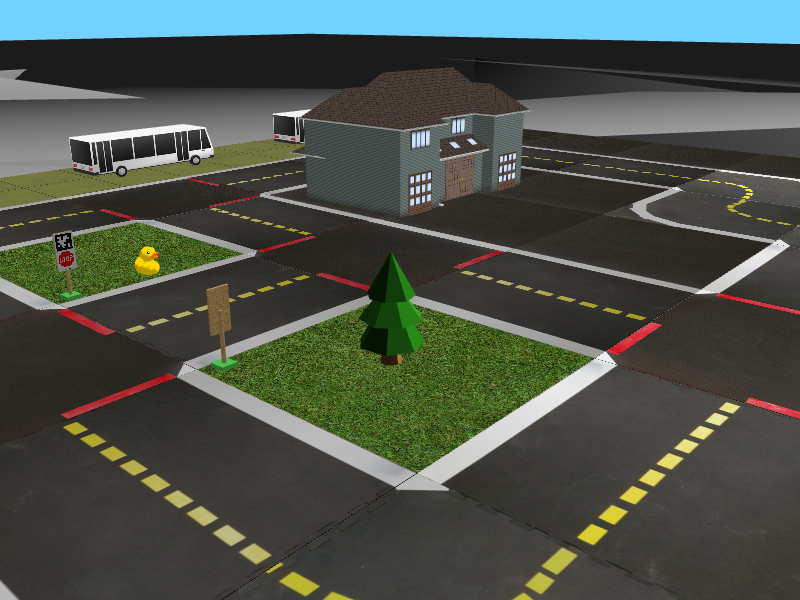
\includegraphics[height=0.5\textheight]{../imgs/gym_duckietown.png}
  \end{figure}
  \vspace{0.5cm}

  \url{https://github.com/duckietown/gym-duckietown}
\end{frame}

\section{Duckievillage}

\begin{frame}
  \frametitle{Duckievillage}

  OpenAI Gym Duckietown com adaptações e exercícios de:
  \vspace{0.5cm}

  \begin{itemize}
    \item Navegação por pontos
    \item Mapa topológico
    \item Campo potencial
    \item Localização
    \item Aprendizagem por imitação
    \item Aprendizagem por reforço
  \end{itemize}
  \vspace{0.5cm}

  \url{https://github.com/RenatoGeh/duckievillage}
\end{frame}

\begin{frame}
  \frametitle{Setup}

  \begin{enumerate}
    \item \href{https://github.com/RenatoGeh/duckievillage}{Instalar Gym-Duckietown com todas as
      dependências}
    \item \texttt{git clone} Duckievillage:
      \begin{itemize}
        \item \scriptsize\texttt{git clone https://github.com/RenatoGeh/duckievillage}
      \end{itemize}
    \item Teste Duckievillage:
      \begin{itemize}
        \item \texttt{cd duckievillage}
        \item \texttt{python3 -m assignments.manual}
      \end{itemize}
  \end{enumerate}
\end{frame}

\end{document}
